\documentclass[a4paper]{article}
\usepackage{hyperref}
\usepackage{graphicx}

\setlength{\oddsidemargin}{0in}
\setlength{\evensidemargin}{0in}
\setlength{\textwidth}{\paperwidth}
\addtolength{\textwidth}{-2in}
\setlength{\topmargin}{0in}
\setlength{\headsep}{1em}
\setlength{\textheight}{\paperheight}
\addtolength{\textheight}{-2in}
\setlength{\footskip}{2em}
\addtolength{\textheight}{-\footskip}

\newcommand{\Sup}{\mathrm{supp}} % Support of a fuzzy set 

\newtheorem{definition}{Definition}
\newtheorem{theorem}{Theorem}
\newenvironment{proof}{\noindent{\bf Proof:}}{\hfill $\Box$\medskip}
\newcounter{ex}
\newenvironment{example}{\addtocounter{ex}1\paragraph{Example \arabic{ex}}}%
  {\hfill $\bigstar$\medskip}

\title{RDF Mining: Project Overview}
\author{Andrea G. B. Tettamanzi \and Catherine Faron Zucker \and Fabien Gandon\\
  WIMMICS Team\\
  Universit\'e de Nice Sophia Antipolis -- Laboratoire I3S -- INRIA\\
  andrea.tettamanzi@unice.fr, faron@polytech.unice.fr, fabien.gandon@inria.fr}

\begin{document}
  \maketitle

\begin{abstract}
  This document provides an overview of a research project on the extraction
  of knowledge from linked open data, loosely inspired by Karl Popper's
  evolutionary approach to epistemology and bringing together the semantic Web,
  inductive logic programming, possibility theory, and evolutionary algorithms.
\end{abstract}

\section{Introduction}

The Semantic Web has come of age.
The first massive deployment of its concept is the Linking Open Data (LOD) initiative,
which covers but the data layer of the Semantic Web.
RDF is the data model of this basic layer.
As of today, billions of RDF triples are available on the Web. They can be queried
by means of a specialized query language, SPARQL, through a number of SPARQL endpoints.

Now that the LOD is reality, the next question is what to make out of it.
An obvious answer to this question is to extract knowledge from it.
LOD is often considered as a giant knowledge base, not just raw data.
Now that the LOD has reached the status of ``big RDF data,'' we want to analyze
it and extract ``smart data'' from it, i.e., learn knowledge from it.
RDF data may be regarded as an oriented, labeled multigraph.
Therefore, it would appear that general methods and techniques that have been devised
for mining graphs should be relevant to mining linked open data.
Graph mining is the field of data mining that deals with
``mining data that is represented as a graph''~\cite{CookHolder2006}.
Graph mining methods have been successfully applied to a variety of problems, where
knowledge has to be extracted from chemical graphs, bioinformatics data,
Web graphs, and social networks. The main techniques employed in graph mining
are frequent substructure mining, link analysis, graph kernels, and graph grammars.
As a matter of fact, as it will become clear in the next sections,
our work does not focus on the graph structure of the knowledge represented using
the RDF formalism, but on its semantics and on the logical axioms that best describe
that knowledge. The approach we propose should therefore be regarded as complementary
to the general graph mining methods and specific to one kind of graph, namely
a particular family of graph-based knowledge-representation formalisms.

Some preliminary work in this direction has been done, which will be briefly surveyed
in Section~\ref{sec:survey}.
Workshops dedicated to this endeavor have been launched, including
the International Workshop on Knowledge Discovery and Data Mining meets Linked Open Data
({Know@LOD}), whose first edition took place at the 9th Extended Semantic Web Conference in 2012,
with the aim of presenting recent work on statistical schema induction, mapping, and link mining,
the \href{http://keg.vse.cz/dmold2013/}{Data Mining on Linked Data Workshop} (DMoLD),
which was held in 2013 in Prague during the European Conference on Machine Learning
and Principles and Practice of Knowledge Discovery in Databases (ECML/PKDD 2013),
and the International Workshop on Consuming On-Lind Linked Data (COLD),
which had its \href{http://db.uwaterloo.ca/cold2013/}{fourth edition} in 2013,
colocated with the 12th International Semantic Web Conference (ISWC) in Sydney, Australia.

Virtually all the approaches to the automated construction of ontologies on the
basis of RDF facts are based on ideas taken from Inductive Logic Programming
(cf.\ Section~\ref{ILP}). However, as Popper rightly observed~\cite{Popper1935},
there is no such thing as a logic of induction. The approach we propose,
whose main components are illustrated in Figure~\ref{fig:synopsis}, is inspired by
Popper's critical rationalism: hypotheses are generated by a mechanism, namely
evolutionary algorithms, which lays outside of Logic; they are then tested using
a deductive process, just like scientific theories are. Possibility theory is used
to capture what Popper calls the ``truth content'' of the hypotheses.

\begin{figure}
  \begin{center}
    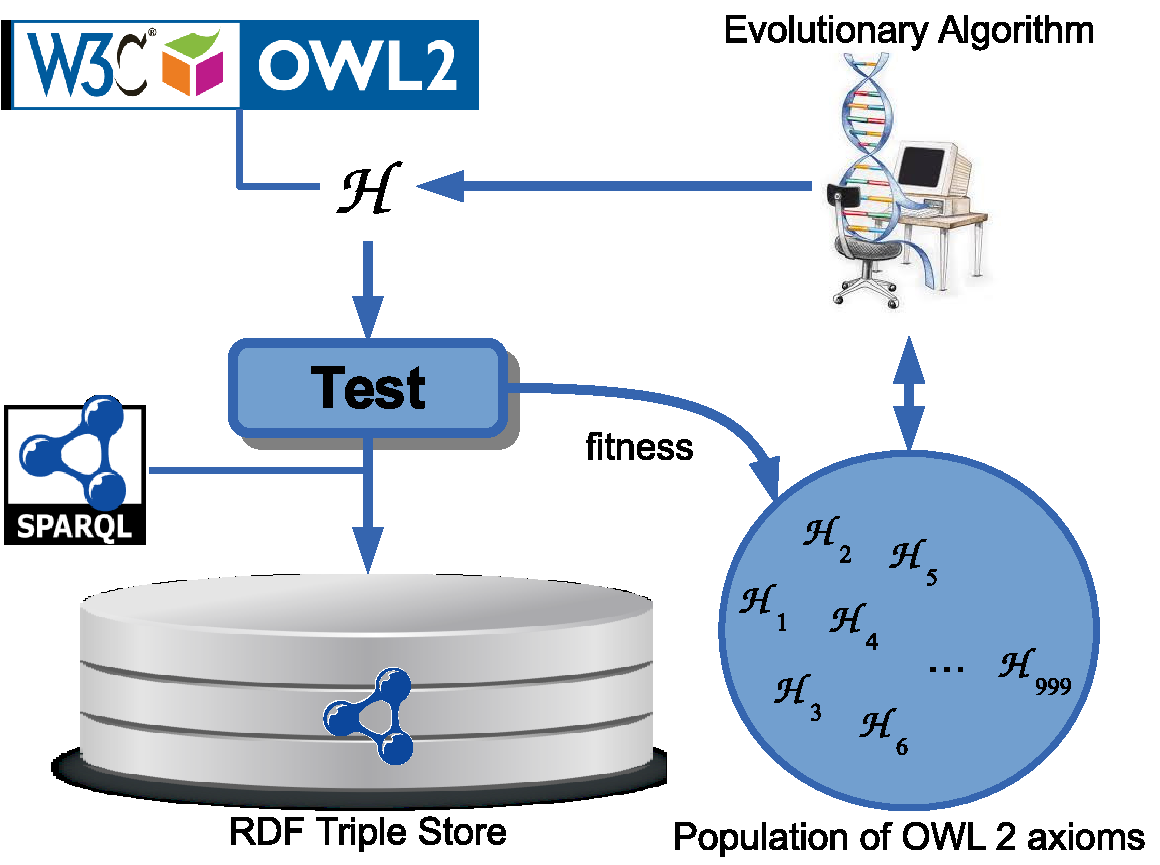
\includegraphics[height=2in]{synopsis}
  \end{center}
  \caption{A schematic illustration of the proposed approach.\label{fig:synopsis}}
\end{figure}



Possible applications of our research are:
\begin{itemize}
\item knowledge extraction from LOD in domains like genomics and proteomics;
\item providing tools to assist in the cleaning and validation of LOD;
\item information intelligence and the monitoring of strategic information on the LOD
  (this is linked with the problem of making sense of weak signals,
  weak signal interpretation).
\end{itemize}

\section{Survey of the Literature}
\label{sec:survey}

An early survey on Semantic Web Mining, dating from 2006, is the article by
Stumme, Hotho and Berendt~\cite{StummeHothoBerendt2006}.
Among the early approaches to what might be generally called ``ontology learning'',
which can go from the simple extraction of schema information all the way to the
induction of description logic TBoxes, we can mention
\begin{itemize}
\item the extraction of RDF schemas by systematic generalization~\cite{DelteilFaronDieng2001};
\item approaches based on clustering~\cite{MaedcheZacharias2002};
\item KAON Text-to-Onto, a framework that supports a semi-automatic, cooperative
  ontology engineering process~\cite{MaedcheStaab2004};
\item approaches based on inductive logic programming~\cite{GrimnesEdwardsPreece2004}.
\end{itemize}

A somehow related task is \emph{ontology alignment} or \emph{mapping},
whose aim is to establish equivalences among concepts defined in independent ontologies.
Extensional (i.e., instance-based) approaches to this task, such as
BLOOMS~\cite{JainHitzlerShethVermaYeh2010}
and BLOOMS+~\cite{JainYehVermaVasquezDamovaHitzlerSheth2011},
or AgreementMaker~\cite{CruzPalmonariCaimiStroe2013}
are of particular interest here.
Indeed, a recent approach to generate alignments between concepts
in ontologies of linked data sources, which looks at not only existing concepts,
but also at new hypothetical concepts defined using conjunctions and
disjunctions of (RDF) types and value restrictions~\cite{ParundekarKnoblockAmbite2012},
is just a little step away from outright ontology learning.
Slightly different approaches are
GLUE~\cite{DoanMadhavanDomingosHalevy2004}
and CSR~\cite{SpiliopoulosValarakosVouros2008},
which make use of machine-learning algorithms to predict the relationships
between concepts and their instances.

After the adoption by the W3C of OWL as an ontology language and of description logics
as its theoretical foundation, a number of approaches have been developed to automatically
identify concepts and produce their descriptions in such formalisms, like
\cite{HellmannLehmannAuer2009}, based on DL-Learner~\cite{Lehmann2009}.
See also Claudia d'Amato's PhD Thesis on similarity-based learning
methods for the Semantic Web~\cite{dAmato2007} and her subsequent work with
Floriana Esposito and Steffen Staab and, in particular DL-FOIL~\cite{FanizziDAmatoEsposito2008}.

Another interesting research direction is to apply statistical schema induction
to enrich the schema of any RDF repository with property axioms. This is what is
done by Johanna V\"olker and colleagues~\cite{FleischhackerVoelkerStuckenschmidt2012},
who use association rule mining methods to induce property axioms in the RL fragment
of OWL (based on the $\mathcal{SROIQ}$ description logic) from RDF datasets.

A statistical approach to inferring RDF triples of the form $x \mathtt{rdf:type} y$
is also presented in \cite{PaulheimBizer2013}, based on the observed statistical
distribution of types in the subject and object positions of other properties.

The integration of traditional Semantic Web techniques and machine-learning-based
statistical inferencing motivates projects like
\href{https://files.ifi.uzh.ch/ddis/oldweb/ddis/research/completed-projects/semweb/sparql-ml/}{SPARQL-ML} \cite{KieferBernsteinLocher2008}.

\section{Targets for Inductive Learning in RDF Mining}

There are many possible targets (i.e., things to learn) for inductive learning from RDF data
which have been addressed in the literature.
These may be classified as concept-centric, property-centric, or instance-centric.

Concept-centric targets include
\begin{itemize}
\item concept induction/discovery;
\item concept subsumption;
\item concept disjointness.
\end{itemize}

Property-centric targets include
\begin{itemize}
\item property induction/discovery;
\item property subsumption;
\item domain restrictions;
\item range restrictions;
\item property disjointness;
\item algebraic properties of RDF properties, such as reflexivity, symmetry, transitivity,
  and functionality.
\end{itemize}

Instance-centric targets include
\begin{itemize}
\item predicting RDF triples in incomplete knowledge bases
(cf., e.g., \cite{DrumondRendleSchmiedtThieme2012}).
\end{itemize}

In addition to the above targets, a very hot current topic in the Semantic Web is
\emph{provenance}, i.e., taking the source of RDF data into account. In this
context, an interesting task would be to mine the RDF triples concerning provenance
to discover, e.g., cultural bias in DBpedia in different languages.

We will adopt as the target of our research the discovery of general OWL~2 axioms,
which may be seen as a generalization of all the learning targets listed above.
This is a very ambitious target and, to achieve it, we will have to combine a wide range
of results and techniques from various areas of machine learning, logic, and philosophy.
In particular, we will exploit ideas from inductive logic programming,
evolutionary computation, possibility theory, and epistemology.

\section{Background Notions from Inductive Logic Programming}
\label{ILP}

Inductive Logic Programming (ILP) is a research area which essentially combines
machine learning with logical knowledge representation to devise a formal framework
and practical algorithms for inductively learning logic programs
(e.g., in languages like Prolog or Datalog) from examples.
A good, if a little outdated, reference to ILP is the book by Lavra\v c and D\v zeroski~\cite{LavracDzeroski1994}; an account of the first twenty years of development of ILP
can be found in \cite{ILPat20}.

The problem of learning logic programs from examples can be viewed as a search problem
in the space of all possible hypotheses. Given a background knowledge, a set of positive
examples and a set of negative examples, expressed in some logical language,
one has to find a hypothesis which covers all positive examples and none of the negative ones.
This problem is NP-hard even if the language to represent hypotheses is propositional logic.
When hypotheses in an expressive language are used, this complexity is combined
with the complexity of evaluating hypotheses.

Although at the beginning the emphasis of ILP was on the inductive synthesis of logic programs,
what defines and unifies most of contemporary ILP is the relational form of the input,
rather than the logical language used to express the output \cite{ILPat20}.
Since ILP underlies most of the research efforts towards the extraction of knowledge from
RDF data, we will recall here some fundamental definitions and results which will be used
as a foundation for building our approach.

\subsection{Coverage}

Intuitively, coverage in ILP is the relationship between a hypothesis and an example,
whereby the example provides evidence in favor of the hypothesis. In that case,
one says that the hypothesis \emph{covers} the example.

Three views on coverage may be distinguished in ILP that are applicable to different
types of data, and ultimately stem from the distinction between the model-theoretic and
proof-theoretic perspectives in logic:
\begin{enumerate}
\item \emph{learning from interpretations} ---
  an example is a logical interpretation $\mathcal{I}$ and an example is covered
  by a hypothesis, which is a logical formula $\phi$, if $\mathcal{I} \models \phi$,
  i.e., $\mathcal{I}$ is a model for $\phi$;
\item \emph{learning from entailment} ---
  an example corresponds to an observation about the truth value of a formula $F$ (a fact)
  and a hypothesis $\phi$ covers the formula $F$ if $\phi \models F$,
  i.e. $\phi$ entails $F$;
\item \emph{learning from proofs} ---
  an example is a proof (or a trace of execution of a logic program)
  and an example $P$ is covered by hypothesis $\phi$ if $P$ is
  a possible proof in the hypothesis $\phi$.
\end{enumerate}
For our purposes, the \emph{learning from entailment} view is the most appropriate:
we have a set of facts, in the form of RDF triples or sets of RDF triples,
and our hypotheses will be formulas in a decidable fragment of first-order logic
(i.e., in a description logic language).

In fact, we will adopt yet another view, which does not fit exactly the orthodox ILP
framework, and stems from our adoption of possibility theory to take data imperfection
into account. We will regard the entire RDF repository as a set of interpretations
(the set of all interpretations $\mathcal{I}$ that agree with all the facts contained in it)
and we will say that a hypothesis is \emph{possible} if there exists a model for it within
that set and \emph{necessary} if all interpretations that agree with the known facts
are models for it. See Section~\ref{possibility-theory} for further details.

\subsection{Structure of the Hypothesis Space}

When hypotheses are logical formulas, the generality relation coincides with that
of logical entailment. A hypothesis $\phi$ is said to be more general than a hypothesis $\psi$
if $\phi \models \psi$. Applying a deductive inference operator leads to specializations,
whereas applying an inverted deductive operator leads to generalizations.
Many generalization and specialization operators have been proposed and theoretically studied
in the framework of ILP and their properties are well understood.

\subsection{Fundamental Techniques}

The hypothesis space can be searched from the bottom up or from the top down.
Generalization techniques proceed from the most specific hypothesis that covers a
given known fact and generalize it until it cannot be further generalized without
covering a counterexample.
Specialization techniques proceed from the most general hypotheses and refine them
until they no longer cover counterexamples.

Generalization and refinement operators will be used in our approach to add intelligent
mutation operators to the evolutionary algorithm in charge of exploring the hypothesis
space (see Section~\ref{EA})

The approach we will propose in the following sections may be classified as a
batch learner that learns multiple predicates; however, it incorporates some aspects
of interactive ILP, because it can be used to build a system that accepts an initial theory,
in the form of an existing ontology, and revises and corrects it based on the contents
of an RDF repository; furthermore, it may use the deductive power of an inference engine
coupled with an existing ontology as an oracle to answer membership queries.

\section{OWL~2 Axiom Discovery}
\label{axiom-discovery}

We choose to use DBpedia, which is a rather rich collection of
facts extracted from the Wikipedia and represented as RDF triples,
as the testbed for devising our approach to axiom discovery.

Why DBPedia? Becuase it poses a number of interesting challenges:
\begin{enumerate}
\item it is one of the largest collections of RDF triples, which covers all possible
  topics; its encyclopedic character makes it a fascinating object of study for a
  knowldege extraction method;
\item due to its collaborative character, it is incomplete and ridden with inconsistencies
  and errors;
\item it is evolutionary: the facts change in time.
\end{enumerate}
Of course, nothing forbid to apply the approach we are developing to more restricted
domains. Examples of such RDF repositories which might be targeted include:
\begin{itemize}
\item the dataset published in RDF by INSEE, the French national bureau of statistics,
  which was one of the targets of the Datalift project, on an analogous dataset
  published by ISTAT, the Italian national bureau of statistics;
\item a genomic or proteomic RDF datasets from Bioportal;
\item RDF data on TV broadcast programs, like those published by the BBC;
\end{itemize}
and possibly others.

Why OWL~2 axioms?
Because we are interested not only in extracting new knowledge from an existing knowledge
base expressed in RDF, but also in being able to inject such extracted knowledge into
an ontology in order to be able to use it to infer its logical consequences.
While the former objective calls for a target language, used to express the extracted
knowledge, which is as expressive as possible, lest we throttle our method,
the latter objective requires using at most a decidable fragment of first-order logic
and, possibly, a language which makes inference problems tractable.
OWL~2 represents a good compromise between these two objectives and one which, in addition,
is standardized and promotes interoperability with different applications.
Furthermore, depending on the applications, it will be possible to select an appropriate
\emph{profile} (corresponding to a different language fragment) exhibiting the
desired trade-off between expressiveness and computational complexity.

\subsection{Generating Hypotheses}

The first step is to generate hypotheses, in the form of OWL~2 axioms.
The generated axioms may be general OWL~2 axioms or be restricted to a particular
fragment (called a \emph{profile}), depending on their intended use once they
are discovered.

The syntax of the logical language from which the axioms are to be
generated is given by a functional-style grammar expressed in the
\href{"http://www.w3.org/TR/2012/REC-owl2-syntax-20121211/#BNF_Notation}{extended BNF notation}
used by the \href{http://www.w3.org/}{W3C}.

The W3C tecnical recommendation \href{http://www.w3.org/TR/owl2-profiles}{OWL~2
Web Ontology Language Profiles} contains the productions of the functional-style syntax
that specify three \emph{profiles} (i.e., fragments) of the OWL~2 language,
namely, OWL 2 EL, OWL 2 QL, and OWL 2 RL.

Not all of the productions contained in the official W3C grammar of OWL~2 need be
considered in order to generate axioms. The reason is here we are not using a grammar
to \emph{define} what a well-formed axiom may be; we are using it to \emph{generate}
axioms that may describe the facts contained in a given RDF tripe store. Therefore,
only resources, literals, properties, and other elements of the language that actually
occur in the RDF repository should be generated.

We solve this issue as follows:
\begin{itemize}
\item a \emph{static} grammar, containing high-level production rules defining the
  structure of the axioms is loaded from a text file; different grammars may be
  prepared to generate different kinds of axioms; such grammars need not define
  low-level non-terminal symbols, which we will call \emph{primitives};
\item production rules for the primitives are constructed at runtime by querying
  the SPARQL endpoint of the RDF repository; they constitute the \emph{dynamic}
  part of the grammar and ensure that the approach is not left behind as the
  contents of the RDF repository evolve or that different RDF repositories can
  be targeted without having to rewrite the grammar.
\end{itemize}


\subsection{Induction from an Epistemological Perspective}
\label{epistemology}

Discovering axioms from a finite, albeit huge, set of known facts
raises philosophical problems that touch upon the discipline of epistemology.
The task may be regarded as a form of inductive reasoning, in that it proceeds
from particular instances of concepts and relations (the RDF triples)
to broader generalizations (the OWL~2 axioms).
At the same time, machine learning provides the theoretical and practical
framework within which the task of axiom induction from RDF triples
should be addressed algorithmically.

The \emph{problem of induction} is the question whether, or under which conditions,
and to what degree, inductive inferences are justified.
A very influential, if controversial, view on such problem, and one which seems
particularly well-suited to the context of axiom induction from RDF repositories,
is Karl Popper's evolutionary approach to epistemology. As a matter of fact,
we might say that Popper's point of view is that the problem of induction is ill-posed.
His solution to the problem is to reject induction as useless and to propose the principle
of \emph{falsifiability} \cite{Popper1935}, which lies at the foundation of his critical rationalism:
all knowledge is provisional, conjectural, hypothetical---we can never finally
prove our scientific theories, we can merely (provisionally) confirm or
(conclusively) refute them.

In Popper's view, the advance of scientific knowledge is an evolutionary process~\cite{Popper1972}
whereby, prompted by a problem, a number of competing conjectures, or tentative theories,
are proposed and systematically subjected to a process of error elimination,
a rigorous scrutiny, whose aim is to falsify them, i.e., to find facts (observations,
results experiments) that show them to be false.
This process performs a similar function for Science that natural selection performs
for biological evolution. Theories that better survive the process of refutation
are not more true, but rather, more ``fit'', i.e., more suited to solving
the problem at hand.
However,
\begin{quote}
while falsifiability is simple as a logical principle, in practice it is exceedingly
complicated---no single observation can ever be taken to falsify a theory,
for there is always the possibility (a) that the observation itself is mistaken,
or (b) that the assumed background knowledge is faulty or defective \cite{Thornton2013}.
\end{quote}

It should be said that Popper made his proposal within the context of Philosophy of Science
and, within this context, his ideas have later been refined and extended by other
philosphers, like Imre Lakatos, and challenged and superseded by others, like Thomas Kuhn.
However, if we abstract them from the specific context of scientific discovery
and we regard them as a tentative explanation of how knowledge may be expanded
through the observation of facts, their value as a source of inspiration cannot be denied.

Popper introduces the concept of \emph{degree of verisimilitude}, which makes us think
of an attempt at something like possibility theory.
Too bad Popper was not aware of possibility theory, otherwise perhaps he could have used
this tool to describe his ideas.
A confirmation that what Popper calls ``degree of corroboration'' of a hypothesis
is to be regarded as a possibility measure is what Popper writes on Page~19,
item~4, of \cite{Popper1972}, which may be paraphrased as follows:
given a theory $T$ and a sentence $s$ (one of its consequences),
if $T \models s$, $\mathrm{corroboration}(s) \leq \mathrm{corroboration}(T)$
and
\[
  \mathrm{corroboration}(T) = \max_{T \models s} \mathrm{corroboration}(s).
\]

We can equate the axioms generated by our algorithm to conjectures, hypotheses
in Popper's terms, and facts contained in the RDF repository to observations,
``basic statements'' in Popper's terms.

We may define the statement that an observation refutes, or contradicts, a hypothesis
as equivalent to saying that a TBox containing the axiom corresponding to the hypothesis
and an ABox containing the assertion corresponding to the observation make an
inconsistent knowledge base.

While the definition of ``contradicts'' is clear enough not to be subject to debate,
defining what it means to ``confirm'' a hypothesis is much more tricky. This is
of course closely related to Popper's observation that a hypothesis can never be
conclusively confirmed.

The difficulty of finding a satisfactory and intuitive definition of confirmation
is witnessed by Hempel's ``black raven''paradox of confirmation~\cite{Hempel1945}:
if we suppose (i) that a simple universal condition (``all ravens are black'')
is satisfied by joint satisfaction of its antecedent and consequent, and we
also accept (ii) that whatever confirms a statement confirms also all its logical
equivalents (e.g., ``all non-black things are not ravens'') --- the \emph{equivalence hypothesis},
then we must conclude that a blue chair, for example, confirms the hypothesis
that all ravens are black.

The hypothesis ``all ravens are black'' may be
written $\mathsf{Raven} \sqsubseteq \mathsf{Black}$ in a description logic language.
This statement is logically equivalent to $\neg\mathsf{Black} \sqsubseteq \neg\mathsf{Raven}$.
The paradox arises from the fact that an observation of, say, a green apple,
may be taken as a confirmation of the latter statement and, therefore, by the
equivalence of the two statements, also of the hypothesis that all ravens are black,
even though it has nothing to do with ravens!

Although Hempel's solution of the paradox was to accept the paradoxical conclusion
and argue that our intuition is biased by our background knowledge, the most popular
solution is to approach it from a statistical point of view. The key of this solution
is to assign a weight to evidence in terms of the Bayes factor. Deciding whether
$\mathsf{Raven} \sqsubseteq \mathsf{Black}$ is true, rather than its contrary, on the basis
of some observed data $D$ may be stated as a model selection problem in which the two
``models'' may be assessed by the Bayes factor
\begin{equation}
  K = \frac{\Pr(D \mid \mathsf{Raven} \sqsubseteq \mathsf{Black})}{\Pr(D \mid \mathsf{Raven} \not\sqsubseteq \mathsf{Black})}.
\end{equation}
Then, observing a green apple does indeed confirm our hypothesis, but its weight
is much lower than observing a black raven, just because there are so many more non-ravens in the
Universe than ravens and so many colors those object can be of. This argument, which
is known as the Bayesian solution to Hempel's paradox, seems convincing enough,
but it cannot be blindly accepted in all contexts.

In fact, the key argument for rejecting a probabilistic approach (like the Bayesian solutions
or the Carnapian approach) in the specific context of axiom induction from an RDF store
like DBPedia, which contains facts automatically extracted from Wikipedia,
which is the result of a collaborative effort, whose coverage is not planned and
subject to cultural and historical biases.
% Catherine: what is specific? Isn't it the case of all any data/knowledge base?
% If we speak about the entire LOD this may be different but this is not the case I suppose
Therefore, there is no reason to assume that the facts contained in an RDF triple store
be \emph{representative} of all possible facts that could be recorded, unless
that RDF store is the result of a planned and well-designed effort aimed at building
a knowledge base providing uniform coverage of a given domain.
Indeed, to use the number of facts supporting a hypothesis
to estimate its probability one would have to make the very strong assumption
that the finite number of recorded facts are randomly extracted, according to a
uniform distribution, from the infinite number of all ``real'' facts, whatever
this means. Adopting a probabilistic approach whereas its assumptions are not
fulfilled might lead to fallacious results.

Applying Popper's idea of falsifiability to the induction problem,
Scheffler and Goodman introduced the concept of \emph{selective confirmation}
\cite{SchefflerGoodman1972}, whereby evidence may be characterized
not simply as satisfying a hypothesis, but, further, as favoring the hypothesis
rather than its contrary.
Thus, evidence of a black raven \emph{selectively confirms} the hypothesis
$\mathsf{Raven} \sqsubseteq \mathsf{Black}$ because it fails to confirm its
negation, $\top \sqsubseteq \mathsf{Raven} \sqcap \neg\mathsf{Black}$, namely
that there exist ravens that are not black. On the contrary, the observation of
a green apple does not contradict $\mathsf{Raven} \sqsubseteq \mathsf{Black}$,
but it does not disconfirm $\top \sqsubseteq \mathsf{Raven} \sqcap \neg\mathsf{Black}$
either; therefore, it does not selectively confirm $\mathsf{Raven} \sqsubseteq \mathsf{Black}$.
Selective confirmation is a nice example of a definition of ``provides evidence in favor of,''
which does not coincide with or imply ``increases the probability of''.
Therefore, we will adopt such a definition of confirmation.

\subsection{Testing Hypotheses}

Conceptually, one could imagine generating all possible OWL~2 axioms (or axioms of
one of the OWL fragments) one by one,
checking each of them against the facts contained in the RDF repository (the ABox).
Of course, we should first complete the TBox with all the axioms that can be
logically inferred from the ones declared in the TBox by taking into account OWL~2 semantics.
Checking an axiom involves constructing one or more corresponding SPARQL queries,
as explained below, executing them and counting the number of confirmations and counterexamples.

This idea of testing OWL axioms is somehow related with approaches aiming at evaluating
the quality of linked data by regarding OWL axioms as integrity constraints.
Clarck and Parsia's Pellet integrity constraint validator (ICV) translates OWL integrity constraint
ontologies into SPARQL queries automatically to validate RDF data~\cite{SirinTao2009}.
A similar approach also underlies the idea of test-driven evaluation of linked data
quality~\cite{KontokostasWestphalAuerHellmannLehmannCornelissen2014}.
To this end, OWL ontologies are interpreted under the closed-world assumption and
the weak unique name assumption. OWL is, therefore, used as an RDF schema language.

What we want to do is the exact opposite: instead of starting from the \emph{a priori}
assumption that a given ontology is correct and verify whether the facts contained
in an RDF base satisfy it, we treat ontologies (and their axioms) like hypotheses and develop
a methodology to verify whether the RDF facts corroborate or falsify them under the
open-world assumption and without making the unique name assumption.

Once a hypothesis is ``accepted'' (considered to be true, or, as Popper would say, the best
available approximation to truth),
it may modify the result of another query testing another hypothesis.
It can also enable to logically infer new axioms in the TBox.
However appealing the idea of automatically extending an ontology may appear,
one should be aware of the dangers: permanently accepting an incorrect axiom and adding
it to an existing ontology might have far-reaching consequences on the subsequent search
for other axioms. One should never forget that all knowledge discovered from RDF data
is conjectural in character and has to be subjected to revision each time that the data
in the RDF repository change or better (i.e., more general, more precise, more falsifiable)
axioms are discovered.

OWL~2 provides for 32 types of axioms and
we may refer to the OWL~2 direct semantics~\cite{OWL2-direct-semantics}
\footnote{\url{http://www.w3.org/TR/2012/REC-owl2-direct-semantics-20121211/}}
for a model-theoretic semantics of all the types of axioms, compatible with
the description logic $\mathcal{SROIQ}$~\cite{HorrocksKutzSattler2006}.

Here is how we intend to use such semantics to check axioms.
A model-theoretic semantics defines a valuation function
$\cdot^\mathcal{I}$ which maps well-formed formulas of the logical language into
elements and sets of elements of the interpretation domain $\Delta^\mathcal{I}$.
We will take the set of all the resources that occur in a given RDF store
(for instance, DBpedia) as the interpretation domain and checking an axiom
will amount to checking whether the interpretation $\mathcal{I}$ with the
valuation function defined by the semantics and the domain given by the
RDF store is a model of the axiom.

However, unlike interpretations, RDF stores, or ABoxes, are incomplete and
possibly noisy. The open-world hypothesis must be made; therefore, absence of
supporting evidence does not necessarily contradict an axiom, and an axiom might
hold even in the face of a few counterexamples (exceptions or possible mistakes).
We will tackle this issue in Section~\ref{possibility-theory}.

\subsection{Translating OWL~2 Expressions into SPARQL Graph Patterns}

We define a mapping $Q(E, x, y)$ from OWL~2 expressions to SPARQL graph patterns,
where $E$ is an OWL~2 expression, $x$ and $y$ are formal parameter which can take up
the name of a SPARQL variable, a resource identifier, or a literal as value,
such that the query
\begin{tabbing}
\texttt{SELECT DISTINCT ?x ?y} \\
\texttt{WHERE \{}\\
\quad $Q(E, \mbox{\tt ?x}, \mbox{\tt ?y})$\\
\texttt{\}}
\end{tabbing}
returns the extension of $E$, i.e., the equivalent of $E^\mathcal{I}$, where,
depending on the nature of $E$, only variable \texttt{?x}
is bound or both \texttt{?x} and \texttt{?y} are bound,
and the queries $\mbox{\tt ASK \{ } Q(E, a, \mbox{\tt ?\_}) \mbox{\tt\ \}}$ and
$\mbox{\tt ASK \{ } Q(E, a, b) \mbox{\tt\ \}}$
check, respectively, whether $E(a)$, with $E$ a class (i.e., concept) expression or
$E(a, b)$, with $E$ a property (i.e., relation) expression.
We will use the \href{http://www.w3.org/TR/sparql11-query/}{SPARQL 1.1 query language}
to write the graph patterns corresponding to OWL~2 expressions.

\subsection{The Reckoning of Evidence}

We take the semantics of the 32 axiom types of OWL~2 as a starting point to define,
for each axiom type, which facts recorded in the RDF triple store are to be taken as
supporting evidence, or \emph{confirmations} of the axiom and which facts are to be
construed as refuting evidence, or \emph{counterexamples}, based on the principles
laid out in Section~\ref{epistemology}.
How such positive and negative evidence should be used to evaluate an axiom
will then make the subject of Section~\ref{possibility-theory}.

Quite obviously, resource names occurring in RDF triples will be regarded as
individual names from the point of view of the model-theoretic semantics taken as
a basis for defining evidence. For the sake of clarity, we will make the explicit
assumption that an RDF resource name (= individual name) is mapped by the interpretation
function $\mathcal{I}$ to exactly one element of the interpretation domain $\Delta^\mathcal{I}$
(this follows trivially from the fact that $\mathcal{I}$ is a function);
however, the same element of $\Delta^\mathcal{I}$ may be referred to by more than one
RDF resource name and any two resource names may potentially refer to the same element.
To be even more explicit, synonyms may exist in an RDF triple store, above and beyond
those that are stipulated by \textsf{owl:sameAs} and other equivalent properties.
This assumption reflects indeed what is the actual state of affairs in the LOD cloud.
An immediate consequence of it is that, given two individual names $a$ and $b$,
$a \neq b$ (i.e., $a$ and $b$ are \emph{syntactically} different) is not sufficient,
by itself, to deduce $a^\mathcal{I} \neq b^\mathcal{I}$, or, equivalently, $a \not\doteq b$
(i.e., $a$ and $b$ do not refer to the same entity).



\section{Possibilistic Evaluation of Axioms}
\label{possibility-theory}

We propose here two functions for evaluating the possibility and the necessity of
an axiom which try to model the basic intuition behind this process in light of
the discussion provided in Section~\ref{epistemology}.
Of course, alternative proposals are possible and we do not claim that ours is the best or
the only one.

Since any RDF repository is a closed set of facts, but the open-world hypothesis
holds, the knowledge base represented by the RDF repository is incomplete.
Moreover, given the heterogeneous and collaborative character of the linked open data,
some facts in the RDF repository may be erroneous; therefore, there is uncertainty,
although not probabilistic in nature. That is why possibility theory is justified
choice as a framework for describing the knowledge extracted from an RDF repository.

\subsection{Possibility Theory}
\label{PossibilityTheory}

Possibility theory \cite{Zadeh1978} is a mathematical theory of epistemic uncertainty.
Given a finite universe of discourse $\Omega$, whose elements $\omega\in\Omega$
may be regarded as events, values of a variable, possible worlds, or states of affairs,
a possibility distribution is a mapping $\pi: \Omega \to [0, 1]$,
which assigns to each $\omega$ a degree of possibility ranging from 0 (impossible,
excluded) to 1 (completely possible, normal).
A possibility distribution for  which there exists a completely possible state of
affairs ($\exists \omega^*: \pi(\omega^*) = 1$) is said to be \emph{normalized}.

There is a similarity between possibility distribution and probability 
density. However, it must be stressed that $\pi(\omega) = 1$ just means that
$\omega$ is a plausible (normal) situation and therefore should not be excluded.
A degree of possibility can then be viewed as an upper bound of a degree of probability.
Possibility theory is suitable to represent incomplete knowledge while 
probability is adapted to represent random and observed phenomena. 
We invite the reader to see~\cite{dubois1991} for more informations
about the relationships between fuzzy sets, possibility, and probability 
degrees.

A possibility distribution $\pi$ induces a \emph{possibility
measure}\index{possibility measure} and its dual \emph{necessity
measure}\index{necessity measure}, denoted by $\Pi$ and $N$
respectively. Both measures apply to a set $A \subseteq\Omega$ (or to a
formula $\phi$, by way of the set of its models, $A = \{\omega : \omega \models \phi\}$),
and are defined as follows:
\begin{eqnarray}
  \Pi(A) &=& \max_{\omega\in A} \pi(\omega); \\
  N(A)   &=& 1 - \Pi(\bar{A}) = \min_{\omega\in \bar{A}} \{1 - \pi(\omega)\}.
\end{eqnarray}
In words, the possibility measure of $A$ corresponds to the
greatest of the possibilities associated to its elements; conversely,
the necessity measure of $A$ is equivalent to the impossibility of
its complement $\bar{A}$.

A few properties of possibility and necessity measures 
induced by a normalized possibility distribution on a finite universe of
discourse $\Omega$ are the following. For all subsets $A, B\subseteq \Omega$:
\begin{enumerate}
  \item $\Pi(A \cup B) = \max\{\Pi(A), \Pi(B)\}$;
  \item $\Pi(A \cup \bar A) = \max\{\Pi(A), \Pi(\bar A)\}=1$;
  \item $\Pi(\emptyset) = N(\emptyset) = 0$,\quad $\Pi(\Omega) = N(\Omega) = 1$;
  \item $N(A \cap B) = \min\{N(A), N(B)\}$;
  \item $\Pi(A) = 1 - N(\bar{A})$ (duality);
  \item $N(A) \leq \Pi(A)$;
  \item $N(A) > 0$ implies $\Pi(A) = 1$;
  \item $\Pi(A) < 1$ implies $N(A) = 0$.
\end{enumerate}
A consequence of these properties is that $\max\{\Pi(A), \Pi(\bar{A})\} = 1$.
In case of complete ignorance on $A$, $\Pi(A) = \Pi(\bar{A}) = 1$.

\subsection{Possibility and Necessity of an Axiom}

The basic principle for establishing the possibility of a formula $\phi$ should be
that the absence of counterexamples to $\phi$ in the RDF repository means $\Pi([\phi]) = 1$,
i.e., that $\phi$ is completely possible.

In general, we may say that a hypothesis should be regarded as all the more
\emph{necessary} as it is explicitly supported by facts and not contradicted by any fact;
all the more \emph{possible} as it is not contradicted by facts.
In other words, given hypothesis $\phi$, $\Pi(\phi) = 1$ if no counterexamples are found;
as the number of counterexamples increases, $\Pi(\phi) \to 0$ strictly monotonically;
$N(\phi) = 0$ if no confirmations are found; as the number of confirmation increases
and no counterexamples are found, $N(\phi) \to 1$ strictly monotonically.
Notice that a confirmation of $\phi$ is a counterexample of $\neg\phi$
an that a counterexample of $\phi$ is a confirmation of $\neg\phi$.

Popper's definition of the \emph{content} of a theory is the set of its logical consequences.
The \emph{relative content} is the set of logical consequences of the theory
given some background knowledge minus all the logical consequences of the
background knowledge (Cf.~\cite{Popper1972}, Page~49 ff.).

For each axiom type $T$, we define a \emph{basic statement} for $T$ as a minimal
ground formula, whose atomic formulas are of the form $C(a)$ or $R(a, b)$,
where $a$ and $b$, $C$, and $R$ are, respectively, an individual name,
an individual name or a literal, a class name,
and a property name occurring in the given RDF store, instantiating the semantics
of axiom type $T$ and thus capable of falsifying an axiom of type $T$.
For instance, basic statements for \textsf{SubClassOf} axioms (of the form $C \sqsubseteq D$)
are all formulas of the form $C(a) \Rightarrow D(a)$, with $a$, $C$, and $D$,
respectively, an individual name and class names occurring in the given RDF store.
We will denote by $\mathrm{BS}_T$ the set af all basic statements for $T$
and by $\mathrm{BS} = \bigcup_T \mathrm{BS}_T$ the set of all basic statements
for the RDF store at hand.

Since an RDF store contains a finite number of triples, only a finite number of
individual, class, and property names and literals can occur in it. Furthermore, the semantics
of all OWL~2 axiom is expressed by a formula constructed from a finite number of
atomic formulas. Therefore, for all axiom type $T$, $\mathrm{BS}_T$ is finite
and so is $\mathrm{BS}$.

Let $\phi$ be an axiom that we wish to evaluate (i.e., a theory).
We define the \emph{content} of an axiom $\phi$ that we wish to evaluate
as the set of its logical consequences, but we restrict it to basic statements, 
to ensure finiteness and testability:
\begin{equation}\label{eq:content}
  \mathrm{content}(\phi) = \{\psi : \phi \models \psi\} \cap \mathrm{BS}.
\end{equation}
The cardinality of $\mathrm{content}(\phi)$ is finite, because $\mathrm{BS}$ is finite,
and every formula $\psi \in \mathrm{content}(\phi)$ may be tested by means of a
SPARQL \texttt{ASK} query, because it is a basic statement.

Let $B$ be some ``background knowledge'' (a set of accepted axioms, or an existing ontology).
Then we may define the content of $\phi$ relative to $B$ as
\begin{equation}\label{eq:relative-content}
  \mathrm{content}(\phi \mid B) = \{\psi : B \cup \{\phi\} \models \psi \mbox{ and } B \not\models \psi\} \cap \mathrm{BS}
  = \mathrm{content}(B \cup \{\phi\}) \setminus \mathrm{content}(B).
\end{equation}
Now, the \emph{truth content} of $\phi$ relative to $B$ is the subset
of $\mathrm{content}(\phi \mid B)$ which is true and the \emph{falsity content}
of $\phi$ relative to $B$ is the subset of $\mathrm{content}(\phi \mid B)$ which
is false.
For instance, if $\phi = C \sqsubseteq D$, $\mathrm{content}(\phi)$ will include
all the facts of the form $C(x) \Rightarrow D(x)$, where $x$ may be replaced by
any individual in the ABox.

Let us define $u_\phi = \|\mathrm{content}(\phi)\|$ as the cardinality of the
set of facts that are a consequence of $\phi$, i.e., of its potential falsifiers.
For the axiom $C \sqsubseteq D$, it would be $u_{C \sqsubseteq D} = \|C^\mathcal{I}\|$.
This is like a universe of discourse when all we are interested in is to establish
whether hypothesis $\phi$ should be accepted or rejected.
In a sense, we may regard $u_\phi$ as an index of what Popper calls the \emph{boldness}
of theory $\phi$.

Let then $u_\phi^+$ be the number of confirmations and $u_\phi^-$ the number of counterexamples
that are actually found in the RDF repository.
Notice that $u_\phi^+$ will be at most the cardinality of the truth content of $\phi$,
while $u_\phi^-$ will be at most the cardinality of the falsity content of $\phi$.
A few interesting properties of these three cardinalities are:
\begin{enumerate}
\item $u_\phi^+ + u_\phi^- \leq u_\phi$;
\item $u_\phi^+ = u_{\neg\phi}^-$;
\item $u_\phi^- = u_{\neg\phi}^+$;
\item $u_\phi = u_{\neg\phi}$.
\end{enumerate}

Here are a few postulates, based on our previous discussion, the possibility
and necessity functions should obey:
\begin{enumerate}
\item $\Pi(\phi) = 1$ if $u_\phi^- = 0$;
\item $N(\phi) = 0$ if $u_\phi^- > 0$ or $u_\phi^+ = 0$;
\item let $u_\phi = u_\psi$; then $\Pi(\phi) > \Pi(\psi)$ iff $u_\phi^- < u_\psi^-$;
\item let $u_\phi = u_\psi$; then $N(\phi) > N(\psi)$ iff $u_\phi^+ > u_\psi^+$ and $u_\phi^- = 0$;
\item let $u_\phi = u_\psi = u_\chi$ and let $u_\psi^- < u_\phi^- < u_\chi^-$: then
  \[
    \frac{\Pi(\psi) - \Pi(\phi)}{u_\phi^- - u_\psi^-} > \frac{\Pi(\phi) - \Pi(\chi)}{u_\chi^- - u_\phi^-},
  \]
  i.e., the first counterexamples found to an axiom should determine a sharper decrease
  of the degree to which we regard the axiom as possible than any further counterexamples,
  because these latter will only confirm our suspicions and, therefore, will provide
  less and less information;
\item let $u_\phi = u_\psi = u_\chi$ and $u_\psi^- = u_\phi^- = u_\chi^- = 0$,
  and let $u_\psi^+ < u_\phi^+ < u_\chi^+$: then
  \[
    \frac{N(\phi) - N(\psi)}{u_\phi^+ - u_\psi^+} > \frac{N(\chi) - N(\phi)}{u_\chi^+ - u_\phi^+},
  \]
  i.e., in the absence of counterexamples,
  the first confirmations found to an axiom should determine a sharper increase
  of the degree to which we regard the axiom as necessary than any further confirmations,
  because these latter will only add up to our acceptance and, therefore, will provide
  less and less information.\footnote{Cf.\ Popper in the English version of
  \cite{Popper1935}, \S83, 2nd paragraph:
  ``When trying to appraise the degree of corroboration of a theory
    we may reason somewhat as follows. Its degree of corroboration
    will increase with the number of its corroborating instances.
    Here we usually accord to the first corroborating instances far greater
    importance than to later ones: once a theory is well corroborated,
    further instances raise its degree of corroboration only very little.''};
\end{enumerate}

A definition of $\Pi$ and $N$ which satisfies the above postulates is, for $u_\phi > 0$,
\begin{eqnarray}
  \Pi(\phi) &=& 1 - \sqrt{1 - \left(\frac{u_\phi - u_\phi^-}{u_\phi}\right)^2}; \\
  N(\phi) &=& \sqrt{1 - \left(\frac{u_\phi - u_\phi^+}{u_\phi}\right)^2},\quad
    \mbox{if $\Pi(\phi) = 1$, 0 otherwise.}
\end{eqnarray}
Notice that this is by no means the only possible definition.

Figure~\ref{fig:poss-nec-plots} shows $\Pi(\phi)$ and $N(\phi)$ as a function of
$u_\phi^-$ and $u_\phi^+$, respectively. The two functions describe an arc of
an ellipse between the minor and the major axis.

\begin{figure}
  \begin{center}
    \begin{tabular}{cc}
      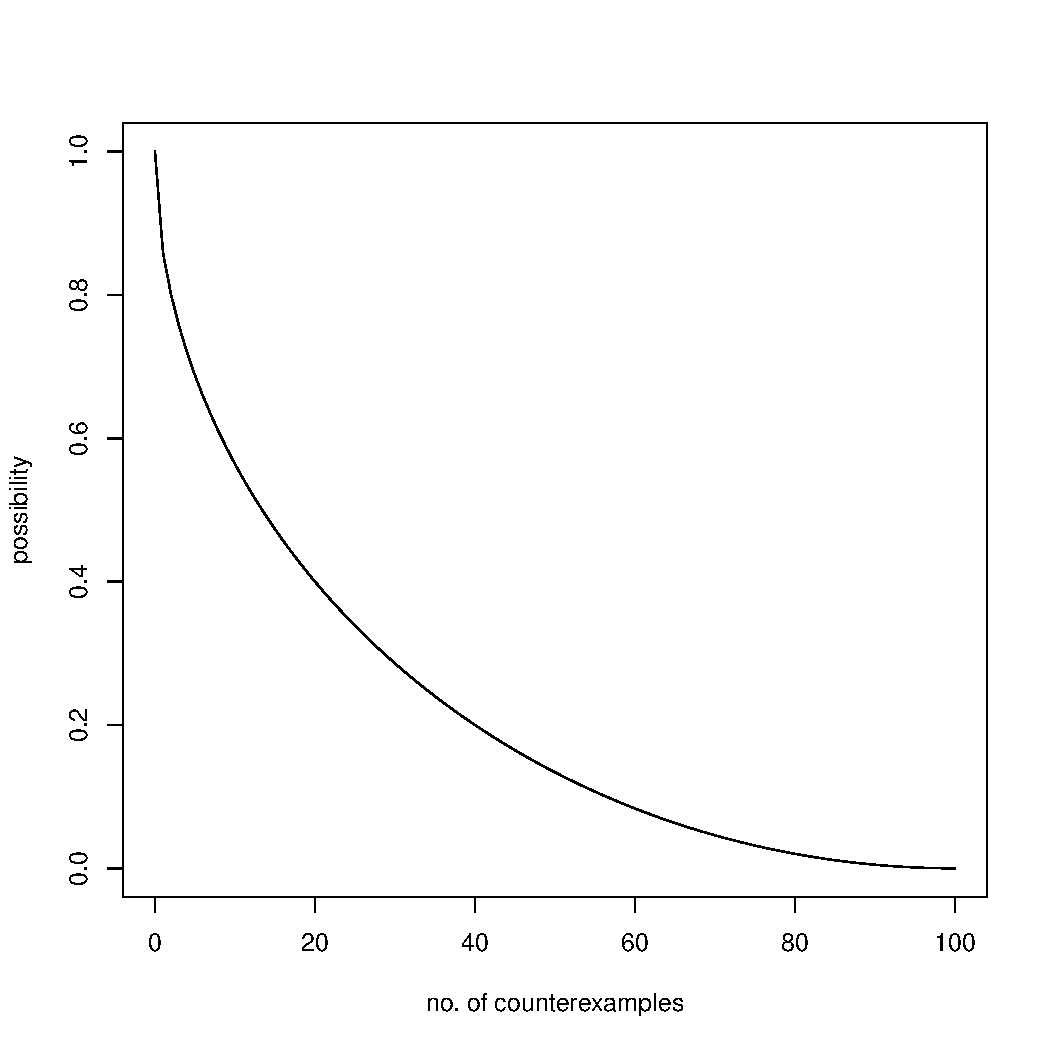
\includegraphics[width=2.5in]{possibility} &
      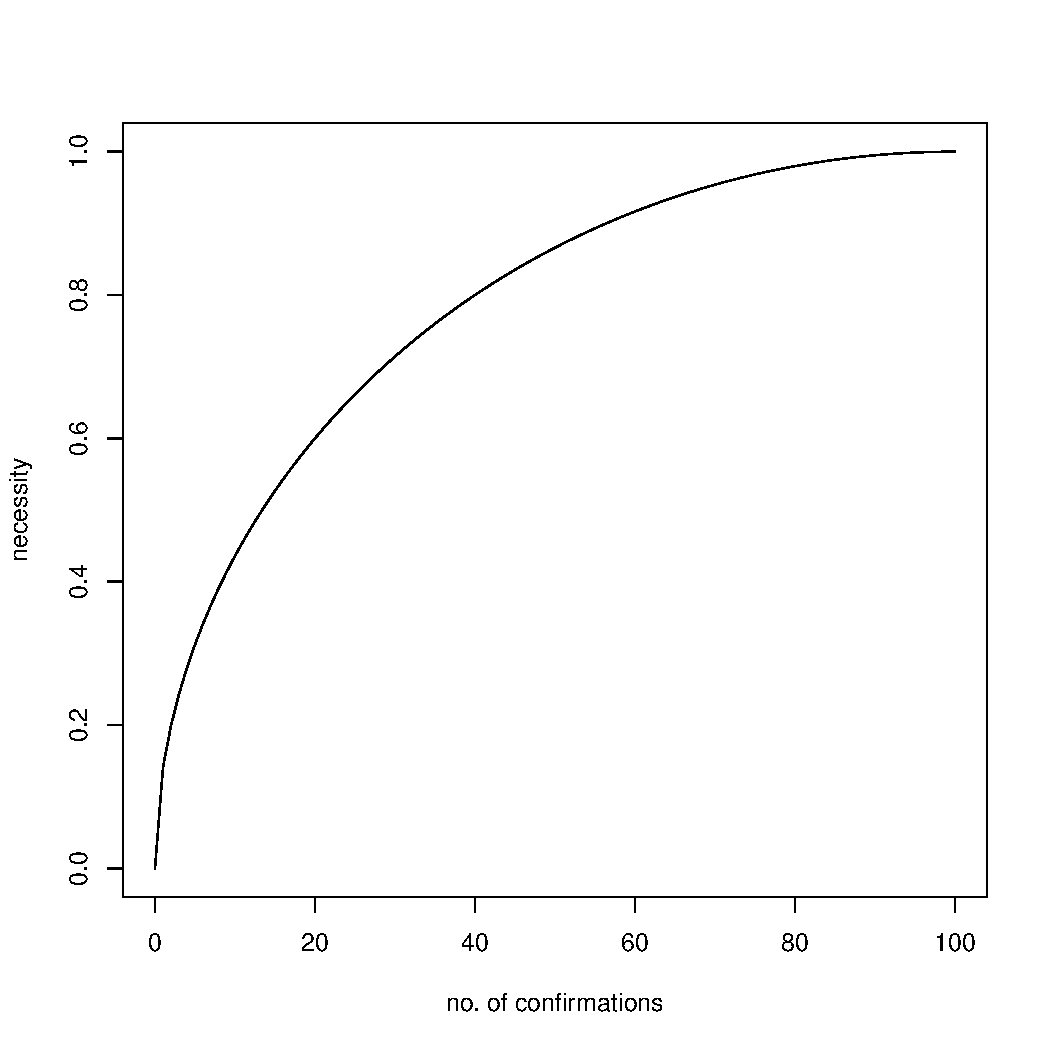
\includegraphics[width=2.5in]{necessity} \\
      (a) & (b)
    \end{tabular}
  \end{center}
  \caption{A plot of $\Pi(\phi)$  as a function of
    $u_\phi^-$ (a) and of $N(\phi)$ as a function of
    $u_\phi^+$ (b) when $u_\phi = 100$.\label{fig:poss-nec-plots}}
\end{figure}

It should be easy tho verify that the above definition satisfies the duality of
possibility and necessity, in that $N(\phi) = 1 - \Pi(\neg\phi)$ and
$\Pi(\phi) = 1 - N(\neg\phi)$.
As a matter of fact, we will seldom be interested in computing the necessity and
possibility degrees of the negation of OWL~2 axioms, for the simple reasons that, in most cases,
the latter are not OWL~2 axioms themselves. For instance, while $C \sqsubseteq D$
is an axiom, $\neg(C \sqsubseteq D) = C \not\sqsubseteq D$ is not.
Notable exceptions are the assertions: \textsf{DifferentIndividuals} is the
negation of \textsf{SameIndividuals}, \textsf{NegativeObjectPropertyAssertion}
is the negation of \textsf{ObjectPropertyAssertion}, and
\textsf{NegativeDataPropertyAssertion} is the negation of \textsf{DataPropertyAssertion}.


\subsection{Probabilistic Score of an Axiom}

An alternative to the possibilistic approach we propose to the evaluation of axioms
which has been used in the framework of knowledge base enrichment is based on probability.
For instance, the approach used by B\"uhmann and Lehmann~\cite{BuehmannLehmann2012}
may be regarded essentially as scoring an axiom by an estimate of the probability
that one of its logical consequences is confirmed (or, alternatively, falsified)
by the facts stored in the RDF repository.

This relies on the assumption of a binomial distribution, which applies when an
experiment (here, checking if a logical consequence of a candidate axiom is confirmed
by the facts) is repeated a fixed number of times, each trial having two possible outcomes
(conventionally labeled \emph{success} and \emph{failure}; here, we might call them
\emph{confirmation}, if the observed fact agrees with the candidate axiom,
and \emph{counterexample}, if the observed fact contadicts it),
the probability of success being the same for each observation,
and the observations being statistically independent.

Estimating the probability of confirmation of axiom $\phi$ just by $\hat{p}_\phi = u_\phi^+/u_\phi$
would be too crude and would not take the cardinality of the content of $\phi$
in the RDF repository into account.
The parameter estimation must be carried out by performing a statistical inference.

One of the most basic analyses in statistical inference is to form a confidence interval
for a binomial parameter $p_\phi$ (probability of confirmation of axiom $\phi$), given
a binomial variate $u_\phi^+$ for sample size $u_\phi$ and a sample proportion $\hat{p}_\phi = u_\phi^+/u_\phi$.
Most introductory statistics textbooks use to this end the Wald confidence interval,
based on the asymptotic normality of $\hat{p}_\phi$ and estimating the standard error.
This $(1 - \alpha)$ confidence interval for $p_\phi$ would be
\begin{equation}\label{eq:Wald}
  \hat{p}_\phi \pm z_{\alpha/2}\sqrt{\hat{p}_\phi(1 - \hat{p}_\phi)/u_\phi},
\end{equation}
where $z_c$ denotes the $1 - c$ quantile of the standard normal distribution.

However, the central limit theorem applies poorly to this binomial distribution
with $u_\phi<30$ or where $\hat{p}_\phi$ is close to 0 or 1.
The normal approximation fails totally when $\hat{p}_\phi = 0$ or $\hat{p}_\phi = 1$.
That is why B\"uhmann and Lehmann~\cite{BuehmannLehmann2012} base their probabilistic score
on Agresti and Coull's binomial proportion confidence interval~\cite{AgrestiCoull1998},
an adjustment of the Wald confidence interval which goes: ``Add two successes and two failures
and then use Formula~\ref{eq:Wald}.'' Such adjustment is specific for constructing
95\% confidence intervals.

In fact, Agresti and Coull's suggestion is a simplification of the Wilson score interval
\begin{equation}
  \left(
    \hat{p}_\phi + \frac{z_{\alpha/2}^2}{2u_\phi} \pm
    z_{\alpha/2}\sqrt{\frac{\hat{p}_\phi(1 - \hat{p}_\phi) + \frac{z_{\alpha/2}^2}{4u_\phi}}{u_\phi}}
  \right) / \left(1 + \frac{z_{\alpha/2}^2}{2u_\phi}\right),
\end{equation}
which is an approximate binomial confidence interval obtained by inverting the approximately
normal test that uses the null, rather than the estimated, standard error.
When used to compute the 95\% score interval, this confidence interval
has coverage probabilities close to the nominal confidence level and can be recommended
for use with nearly all sample sizes and parameter values.

A remark about B\"uhmann and Lehmann's approach is in order.
B\"uhmann and Lehmann only look for confirmations of $\phi$, and treat
the absence of a confirmation as a failure in the calculation of the confidence interval.
This is like making an implicit closed-world assumption. In reality, the probability
of finding a confirmation and the probability of finding a counterexample do not add to one,
because there is a non-zero probability of finding neither a confirmation nor a counterexample
for every potential falsifier of an axiom. Their scoring method should thus be
corrected in view of the open-world assumption, for example by using
$\hat{p}^* = u_\phi^+/(u_\phi^+ + u_\phi^-)$ as the sample proportion instead of $\hat{p}$.

However, there is a more fundamental critique to the very idea of computing the likelihood
of axioms based on probabilities. In essence, this idea relies on the assumption
that it is possible to compute the probability that an axiom $\phi$ is true given
some evidence $e$, for example $e$ = ``$\psi \in \mathrm{content}(\phi)$ is in the RDF repository'',
or $e$ = ``$\psi \notin \mathrm{content}(\phi)$ is in the RDF repository'',
or $e$ = ``$\psi \in \mathrm{content}(\phi)$ is not in the RDF repository'', etc.,
which, by Bayes' formula, may be written as
\begin{equation}
  \Pr(\phi \mid e) =
    \frac{\Pr(e \mid \phi)\Pr(\phi)}{\Pr(e \mid \phi)\Pr(\phi) + \Pr(e \mid \neg\phi)\Pr(\neg\phi)}
\end{equation}
However, in order to compute (or estimate) such probability,
one should at least be able to estimate probabilities such as
\begin{itemize}
\item the probability that a fact confirming $\phi$ is added to the repository
  given that $\phi$ holds;
\item the probability that a fact contradicting $\phi$ is added to the repository
  in error, i.e., given that $\phi$ holds;
\item the probability that a fact confirming $\phi$ is added to the repository
  in error, i.e., given that $\phi$ does not hold;
\item the probability that a fact contradicting $\phi$ is added to the repository
  given that $\phi$ does not hold.
\end{itemize}
Now, it is not hard to argue that the above probabilities may vary as a function of the
concepts and properties involved. Let us take a subsumption axiom $C \sqsubseteq D$
as an example. A fact confirming it is a triple ``$x$ \texttt{a} $D$'', with $x\in C^\mathcal{I}$,
whereas a fact contradicting it is a triple ``$x$ \texttt{a} $C'$'', with $x\in C^\mathcal{I}$
and $C' \sqcap C = \bot$. Assuming that $C \sqsubseteq D$ holds, we may suspect that
a triple ``$x$ \texttt{a} $D$'' is much likely to be found in the repository
if $D$ is either very specific (and thus ``closer'' to $x$) or very general (like
\texttt{owl:Person}), and less likely if it is somewhere in the middle.
This supposition is based on our expectations of what people are likely to say
about $x$: for instance, an average person, if asked ``what is this?'' when pointing
to a basset hound, is more likely to answer ``a dog'' or ``an animal'' than,
say, ``a carnivore'' or ``a mammal'', which, on purely logical grounds,
would be perfectly valid things to say about it.
There is thus an inherent difficulty with estimating the above probabilities,
one which cannot be solved otherwise than by performing a large number of
experiments, whose results, then, would be hard to generalize.
By this argument, any axiom scoring method based on probability or statistics is doomed
to be largely arbitrary and subjective or, in other words, \emph{qualitative}
and therefore hardly more rigorous or objective than our approach based on possibility theory.

\section{Performance Criteria}

Apart from the degree of possibility or necessity, other criteria must be used to
evaluate the merit of an axiom or a set of axioms. In a sense, possibility and
necessity replace the traditional measure of \emph{classification accuracy} which
is used in machine learning.

Other important performance criteria used in machine learning include the following:
\begin{itemize}
\item \emph{transparency}, which denotes the extent to which an axiom is understandable
  to humans; in practice, this can be measured by the syntactic complexity of the axiom,
  such as the number of nodes in its parsing tree;
\item \emph{statistical significance}, measured as the probability
  that the fact that an axiom agrees with the known facts is not due to chance;
\item \emph{information content}, which, roughly speaking, ranks an axiom according
  to the difficulty of the classification problem corresponding to it, e.g., by
  measuring the relative proportion of confirmations or counterexamples with respect
  to all known facts: on one extreme, a tautology is supported by all facts and,
  therefore, it has no information content; an axiom stating that
  a person playing for a soccer club is a soccer player bears more information
  than another axiom saying a person playing for a soccer club is a sportsperson,
  because the evidence supporting the former is harder to find than the evidence
  supporting the latter.
\end{itemize}

\section{Evolutionary Search of the Hypothesis Space}
\label{EA}

This section describes the evolutionary algorithm that is used to explore
the hypothesis space in search of axioms.

\subsection{The Case for Evolutionary Algorithms}

If we cast the problem of ontology induction as an optimization problem,
we will be able to use the global optimization capabilities of evolutionary algorithms.
One way to formulate the problem is the following: given an RDF repository,
find the most specific set of axioms that are satisfied by it.
Here, ``most specific'' should be understood as meaning ``most informative''.

From a possibilistic point of view, each axiom may be assigned a degree of necessity,
which may be regarded as a degree of membership of the axiom in the ontology.
The ontology is thus a fuzzy set of axioms describing the triples in the RDF repository.
We may therefore apply measures of specificity devised for fuzzy sets.

Evolutionary algorithms are parallel in nature, and they exhibit what parallel
computing researchers call \emph{embarrassing} parallelism: under the island model,
a population of evolving individuals may be split into a number of subpopulations
that evolve almost independently, exchanging migrants at time intervals that may be
made large at will. This fact positions evolutionary algorithms among the most
promising techniques to ensure scalability in the face of an ever expanding volume
of RDF triples and to exploit distributed computing resources, which are the norm
on the Web.

Several proposals to use evolutionary algorithms in combinations with ILP started
to appear in the literature at the beginning of the new millennium:
one was presented in~\cite{ReiserRiddle2001} by Philip Reiser, who later ended up working at the
\href{http://en.wikipedia.org/wiki/Robot_Scientist}{Robot Scientist}
platform, one of the flagship projects of the ILP community, and stopped publishing after 2004,
and Patricia Riddle, who is still active in research on evolutionary algorithms.
Federico Divina wrote his PhD dissertation \cite{Divina2004th} on that topic and,
in the process, published with his advisor Elena Marchiori some papers about
learning in first-order logic \cite{DivinaMarchiori2001,DivinaMarchiori2002}
and, more specifically, on handling continuous values \cite{DivinaMarchiori2005}.
He then proposed an evolutionary algorithm for ILP, called ECL
(for Evolutionary Concept Learner) \cite{Divina2010}, which evolves a population of
Horn clauses by repeated selection, mutation and optimization of more fit clauses.
ECL relies on four greedy mutation operators for searching the hypothesis space,
and employs an optimization phase that follows each mutation.
A third line of research was then carried out by Alireza Tamaddoni-Nezhad and
Stephen Muggleton
\cite{TamaddoniNezhadMuggleton2000,TamaddoniNezhadMuggleton2002,TamaddoniNezhadMuggleton2008}.

The rationale for using evolutionary algorithm as a meta-heuristic for ILP is that
they might mitigate the combinatorial explosion generated by the inductive learning
of rich representations, such as those used in first-order logic, but also in description logics.
A critical perusal of appraches aiming to combine evolutionary algorithms with
ILP~\cite{Marginean2003}, however, has uncovered a series of systematic and fundamental
theoretical errors that render those approaches moot. In particular, the binary
representation used by Tamaddoni-Nezhad and Muggleton, far from restoring completeness
to the \textsc{progol} learner's search of the subsumption lattice, is both overwhelmingly
unsound and severely incomplete.

\subsection{Roadmap for the Implementation of an Evolutionary RDF Miner}

The extended BNF grammar of an OWL profile may be used as the underlying grammar for grammatical evolution.
Grammatical Evolution is a system that can be used to automatically generate expressions
in any language; in this case, we are interested in generating individual axioms, which
will be encoded as numerical chromosomes, and collections of axioms, represented
either as multi-chromosome individuals or, more likely, as populations.

A chromosome will thus be decoded into an OWL~2 axiom in functional-style syntax,
which will be used for serialization and internal manipulation;
axioms will be translated to Manchester syntax for user-friendly output;
axioms will also be translated into RDF/XML syntax, if necessary, in order to be exchanged
with any conformant OWL~2 software, such as editors and reasoners.

The fitness of an axiom will measure the extent to which it is supported
by known facts, contained in a triple store accessible via a SPARQL endpoint
(an ABox). This extent will be evaluated based on the semantics of the axiom,
as explained in Sections~\ref{axiom-discovery} and \ref{possibility-theory} above.
In principle, the fitness of axiom $\phi$ should be directly proportional to
its necessity $N(\phi)$, its possibility $\Pi(\phi)$, and its boldness $u_\phi$.
Different definitions of a fitness functions are possible: for instance, one
function might give priority to a bolder theory that is possible but not necessary,
while another might treat all possible but non-necessary theories as equivalent,
independently of their boldness.

Some niching, crowding, or fitness-sharing technique will have to be used
to ensure that a population contains different ``species'' of axioms,
i.e., axioms that cover different aspects of the known facts.
One possible definition of \emph{species} might be ``a consistent set of axioms''.
This would lead to a co-evolutionary approach whereby individuals of different
species compete against each other while individuals of the same species
cooperate to some extent.

Intelligent mutation operators based on ILP generalization and refinement operators
(see Section~\ref{ILP}) will enhance the search capabilities of the evolutionary algorithm.

A prototype system is being developed in Java.
The prototype uses \href{http://jena.apache.org/}{Apache Jena} to interface with
the Linked Data platform and
\href{http://ncra.ucd.ie/Site/GEVA.html}{GEVA v.~2.0},
an implementation of Grammatical Evolution in Java
developed at UCD's Natural Computing Research \& Applications
group~\cite{ONeillHembergGilliganBartleyMcDermottBrabazon2008}
to evolve axioms according to a given BNF functional-style grammar.


\section{Validation}

The key question is: how does one goes about testing and validating an approach
to RDF mining? For simple tasks, like RDF triple prediction, one can use the same
validation protocol as in data mining, performing $k$-fold cross-validation and
looking at the resulting confusion matrix. A sensible alternative, which may be
somehow extended to other RDF mining tasks, is to use the same protocol as in
information retrieval (in fact, here, we are dealing with knowledge retrieval)
and look at precision, recall, and the $F$-measure.
Recall, here, would be the fraction of correct and relevant formulas
(for most tasks, in fact, axioms) discovered.
Precision would be the fraction of the generated formulas that happen to be correct and relevant.
This, of course, supposes to know which are the correct and relevant formulas, which
may not always be the case.
Proposing a well-motivated, principled experimental protocol for the validation
of this and other approaches to RDF mining could be, all by itself, a valuable
contribution by our work.

In general, the approach to validation would be to take a known ontology,
cripple it by removing a certain number of axioms, and check
to what extent the proposed RDF mining method is able to recover them.
This is a first step but it depends on the quality of he original ontology,
i.e., whether it is ``complete'' or not.

Another issue is the comparison to other approaches. A comparison might be carried out
with respect to different aspects.
One is a comparison of the results, i.e., of the knowledge learned with each approach,
evaluated by domain experts.
Another is a comparison of the extent to which each approach is able to recover axioms
removed from an ontology.

\bibliographystyle{plain}
\bibliography{RDFMining}
\end{document}
